\chapter{Conclusions and Future Work}


\section{Conclusions}
Throughout this work, we have advocated for robust, data-driven, computer-vision algorithms which will enable the deployment of autonomous robotics in unconstrained environments. 

In this work we identified an opportunity to address a knowledge gap - namely the ability to perform visual odometry using an uncalibrated camera array. Meanwhile, we have blended the successes of two promising technologies - light field imaging and deep learning - to address the visual odometry problem.  Not only does our proposed algorithm build robustness through experience, but it has been designed to operate on minimal prior knowledge of its parent system, adapting to adverse environments and improving performance \textit{in situ}. 

In this work, we have provided evidence that computational imaging - the co-design of optics and algorithms - will continue to propel advancements in imaging technology for the foreseeable future. Most of us need not look any further than our own pockets to find a piece of technology that is emblematic of the progress computational imaging has made. Since we commenced this work, the typical number of cameras embedded in flagship mobile devices has evidently graduated from two to three (and four in some devices) - which is incidentally enough to acquire a sparse 4D light field.

\subsection{Applications}
We envisage a number of potential applications for our algorithm. Primarily, it has been designed as an odometry component for autonomous systems, simplifying the process of navigation, localisation and mapping. Robotic systems rarely operate in the absence of feedback data, especially in intelligent, mobile systems. Where robotics is concerned, we frequently hear about sensor-fusion - a simple and practical way of combining multiple sources of truth to build the best probabilistic picture of the robot's operating environment. A simple application is hovering-in-place using an AUV in a GPS denied area - a problem that in any practical scenario cannot be solved with dynamic system models alone, requiring some form of feedback data. Feedback using visual odometry is good, but feedback using a fusion of visual odometry and inertial measurements for example would be better. 

\begin{figure}[H]
    \subfloat[iPhone 11 Pro]{
        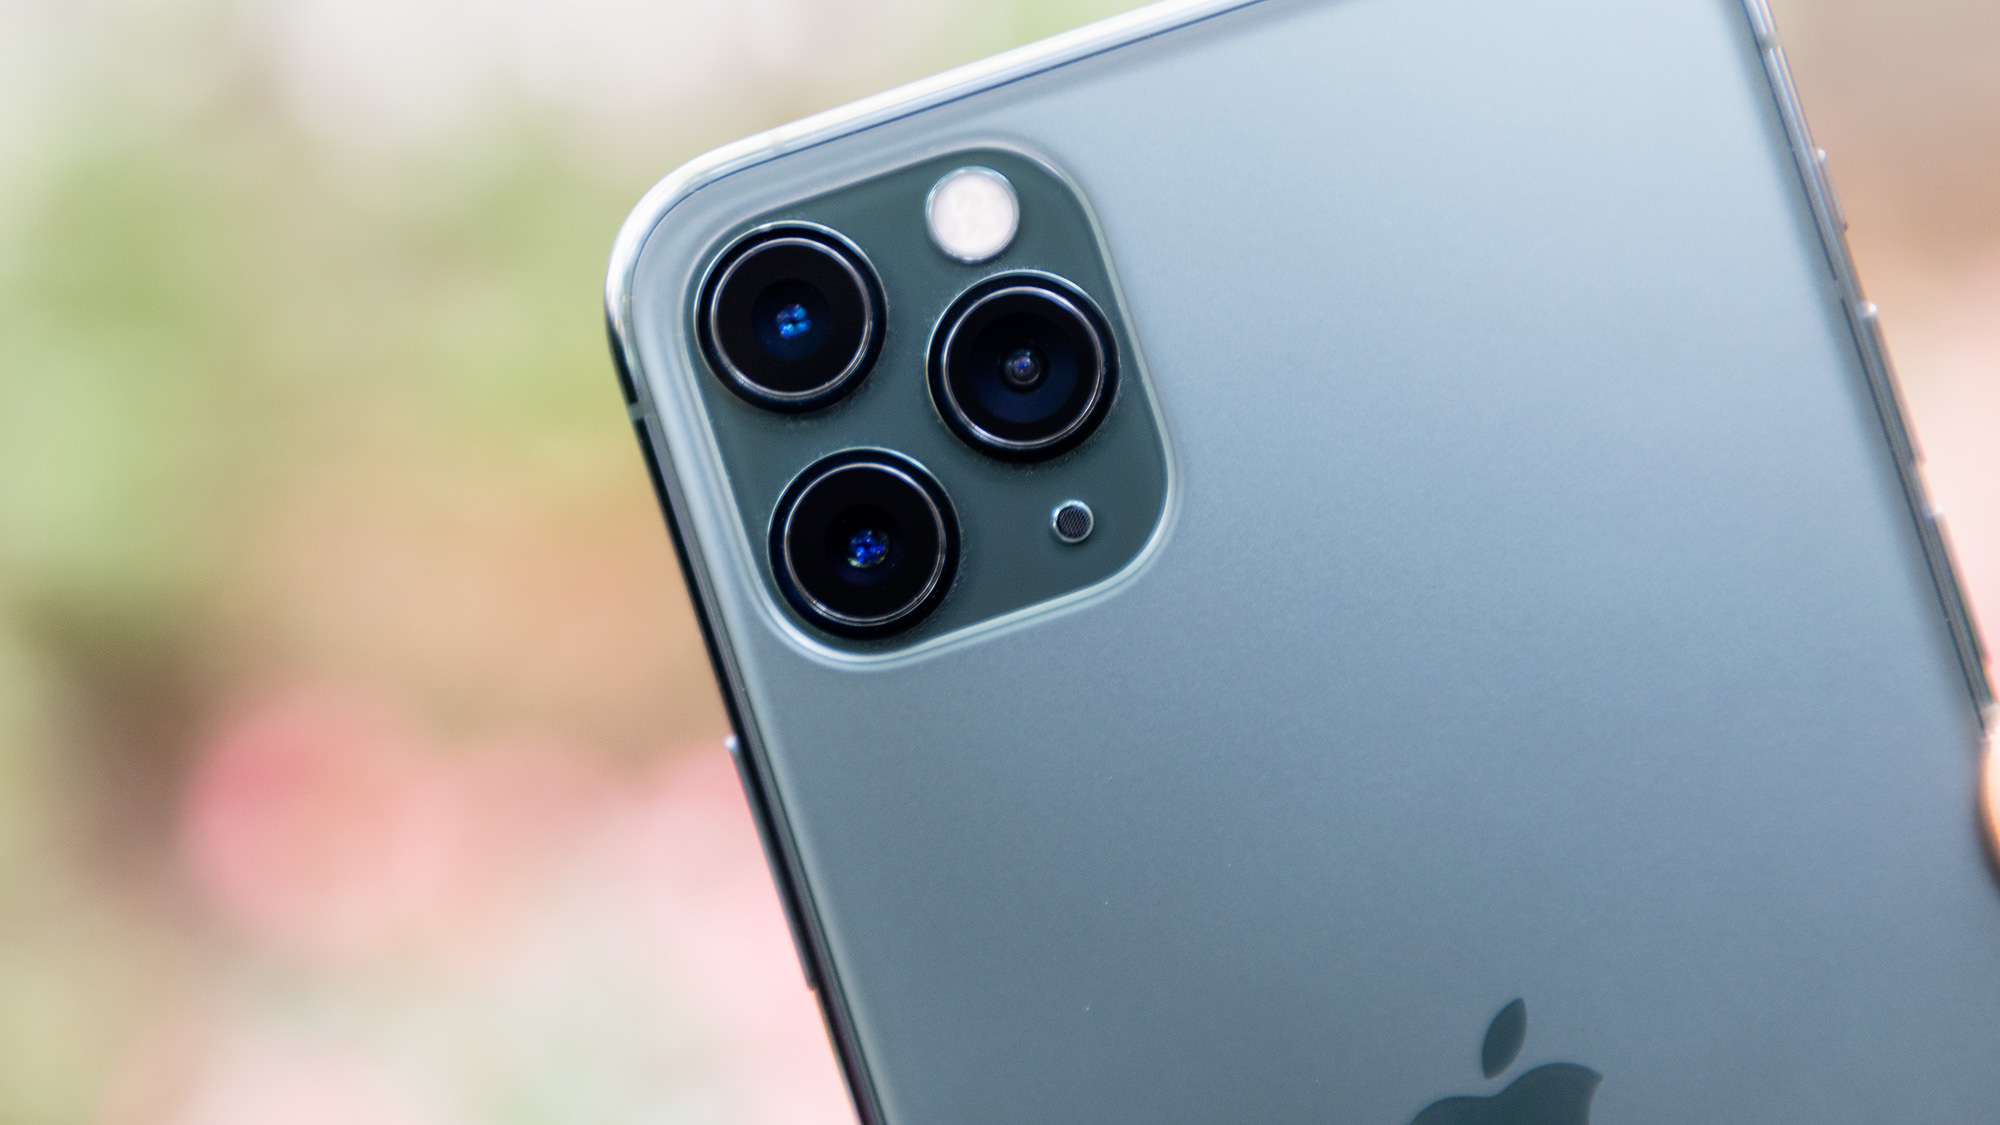
\includegraphics[height=1.2in]{images/iphone11.jpg}
    }
    \subfloat[Samsung Galaxy S20 Ultra]{
        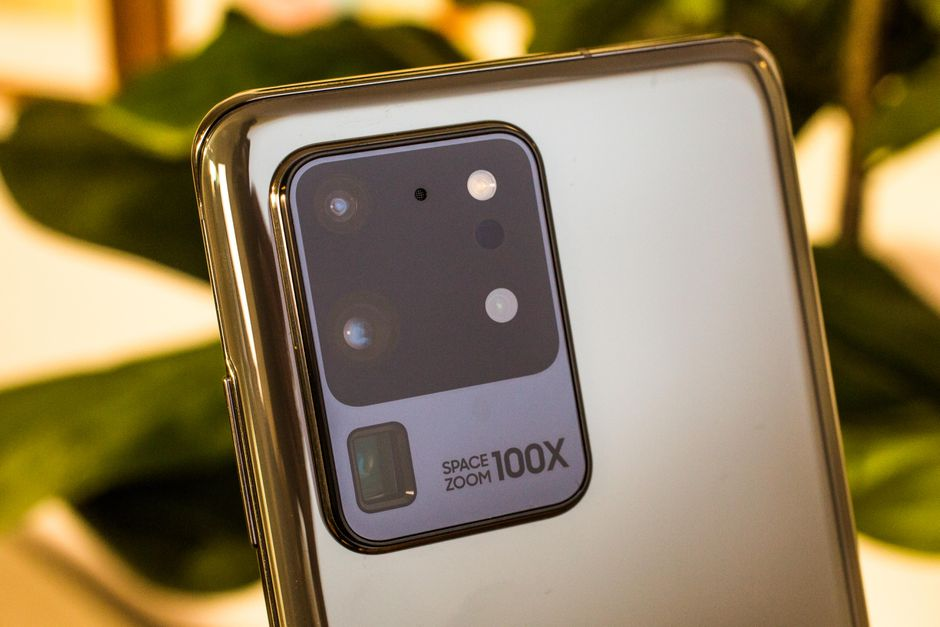
\includegraphics[height=1.2in]{images/s20ultra.jpg}
    }
    \subfloat[Pelican Imaging Camera Array]{
        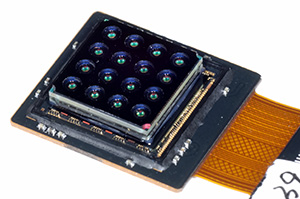
\includegraphics[height=1.2in]{images/pelican.jpg}
    }

    \caption[Examples of multi-view imaging being introduced in consumer devices]{
        Consumer electronics producers are embracing computational imaging, with the number of cameras on many mobile devices now exceeding 3, not only allowing users more control over their photography but enabling those in the computer vision community to continue innovating. 
    }
    
\end{figure}


While we have primarily focused on robotics, we also recognise that as computational imaging becomes more pervasive in consumer electronics, numerous potential applications of our algorithm emerge. For example, the ability to track camera motion while simultaneously reconstructing a 3D model of the scene has applications in Augmented Reality, enabling 3D models to be rendered over the top of a real world scene. Similarly, the ability to predict camera motion from one frame to another may be employed to smooth motion in a shaky video. In a similar vein, video frames may even be interpolated using the photometric warp technique that we have used for training our models - effectively increasing the frame rate of the footage.

\section{Future Work}

There are numerous exciting avenues of research to branch off this work, which we describe in the following. In suggesting these research questions, we begin with more immediate extensions of the present work, and build up to longer-term research goals. 

\subsection{Real-time Inference and Online Learning}
We have suggested throughout this work that our algorithm is capable of online learning. A simple yet exciting extension of this work is to implement a system that is capable of such online learning, perhaps on a mobile robotic platform or visually equipped quad-rotor. Depending on the implementation requirements, this may mean minifying the computational cost of the algorithm to enable training on the edge device, or alternatively modifying the training routine to operate in the cloud whilst collecting data simultaneously from several devices. Deployment options may also be explored - weighing up the comparable advantages of inference at the edge versus in the cloud. Devices such as the Coral \footnote{https://coral.ai/products/dev-board/} and Jetson Nano \footnote{https://developer.nvidia.com/embedded/jetson-nano-developer-kit} have seen `edge' computing rise in popularity, while the scalability of cloud platforms has similarly made their services very popular. 

\subsection{Fusion and Filtering}
Light field imaging is just one expression of computational imaging - meanwhile, RGB-D sensors, lidar and time-of-flight cameras can, and should be used to expand the versatility of our system. Current limitations of our algorithm - such as the challenges presented by low-texture materials - may be partially addressed by the fusion of multiple visual sensors. This makes sense especially in larger robotic platforms such as autonomous vehicles and industrial robotics - where safety and robustness are key. In a similar vein of research, we suggest that integration with existing SLAM algorithms is a useful research direction that will more rapidly enable the adoption of such algorithms in mobile robotics.

\subsection{Deep Learning and Light Field Imaging}
Deep learning is no longer an obscure area of research - software libraries and hardware-accelerated devices are making it more accessible than ever, inviting even the most idly curious to participate. Similarly we have witnessed a maturing of light field technology, with applications in robotics, consumer electronics and industry. Applications which have previously found success applying deep learning to conventional imagery now stand to also benefit from the rich 3D data captured by light field cameras. In combination, these technologies present exciting possibilities, and the potential applications are limited only by their broader adoption, and the ingenuity of the people who use it.